\documentclass[11pt]{jsarticle}

\usepackage{SPR}

\headerSPR
\begin{document}
	\titleSPR{\number\year}{\number\month}{\number\day}{D1}{吉田 皓太郎}
%%%%%%%%%%%%%%%%%%%%%%%%%%%%%%%%%%%%%%
	\articleSPRabst
		\begin{itemize}
			\item 着後形状を評価可能なバストモデルの構築.
		\end{itemize}
		
		
	\articleSPRobj
		\begin{enumerate}
			\item カップ装着時における,着後形状が分かればよい.(着圧に関してはバストよりもベルトの話?の方が大きな要素となる)
			\item バスト外形と重量などの基本的データのみでその力学的なふるまいを再現できる可能性を持っている(?)
		\end{enumerate}
%%%%%%%%%%%%%%%%%%%%%%%%%%%%%%%%%%%%%%
% 1.前回からのノルマ
	\articleSPRitemsone
		%\begin{enumerate}
		%	\item A
		%\end{enumerate}
		
		\tableofcontents
		
		
%%%%%%%%%%%%%%%%%%%%%%%%%%%%%%%%%%%%%%
%\begin{itemize}
%	\item 新規手法について
%	\item ISFAアウトライン
%\end{itemize}
%%%%%%%%%%%%%%%%%%%%%%%%%%%%%%%%%%%%%%
% 2.具体的な成果
	\articleSPRitemstwo
%%%%%%%%%%%%%%%%%%%%%%%%%%%%%%%%%%%%%%
	\section{研究成果}
			\subsection{現状報告}
			超弾性体を対象に,形状最適化を行いました.形状に関する材料パラメータは,以下の表に示すデータを用いた.なお,超弾性体を表すひずみポテンシャル関数には,大ひずみ状態を仮定しないことから,以下に示すようなNeoHooken体を用いた.
			\begin{equation}
				W = c_1(I_C-3) + \frac{1}{D_1}(J-1)^2
			\end{equation}
			
			このようにすることで,$ W $が必ず凸であることを満たすようになる.
			制約条件について述べる.ここで,関連の形状最適化についてを参照するように,ABAQUSでは,解析を行ってからその評価を行って,メッシュを修正する.そのため,解析条件についての制約条件と,最適化についての制約条件を分けて述べる.
			
			まず,解析の際の制約条件には,バストが体と一致している必要があるので,平面固定の制約を用いた.また,荷重は重力のみを作用させている.
			
			次に,最適化についてはバストの外部形状が変わらないという条件を用いた.また,解析時の境界平面上の乳腺形状について,Z軸方向の成長をしないように制約を入れた.
			
			\subsection{問題点}
			ABAQUSのToscaStructureでは,関連にも記載したが,条件ベースのトポロジー最適化と同じアルゴリズムを使用している.詳しい説明が書いてないのでなんとも言えないが,基本的には応力均一になるように,表面メッシュを修正するようなものらしい.また,製品設計の多くの場合では,トポロジー最適化を行ったのちの微修正に用いられることから,大きなメッシュ形状の変更が行われにくいという記載がマニュアルにあった.
			
			この問題を解決するためには,
			\begin{enumerate}
				\item ある程度の初期解を与える手法(こっちのほうが確実かも)の構築
				\item 別の形状最適化手法(力法など)を用いる
			\end{enumerate}
			といった解決策が必要となるかもしれない.
			
			\subsection{関連)形状最適化について}
				形状最適化は,領域最適化という風に言われる場合もあります.その手法は,大きく分かれて2つあります.一つはB-splineなどのいわゆるパラメトリック係数を最適化することで,形状を最適化する手法.もう一つは,有限要素法におけるメッシュの各節点が最適化変数であり,これをある適当な目的関数を最小化/最大化するように変位させるという方法である.(ノンパラメトリック最適化と呼ばれる)
				
				様々な手法が提案されているが,ABAQUSでは,条件ベースのトポロジー最適化と同じアルゴリズムが用いられている(おそらく随伴法設計感度解析であると思われる.)
				\begin{enumerate}
					\item 有限要素法により普通に解析する.
					\item 勾配法的なものに基づいて,移動量の更新的なものを決める.
					\item この更新幅に従って,節点移動の更新が行われる.
					\item 再計算,指定されたサイクルまで続く.
				\end{enumerate}
			\begin{figure}[!h]
				\centering
					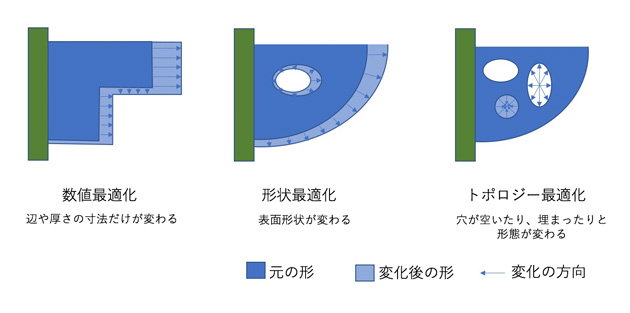
\includegraphics[width=0.8\columnwidth]{Figure/img_opt.jpg}
				\caption{最適化の違い}
				\label{fig:ExampleOfBra_str}
			\end{figure}
		\begin{table}
			\caption{材料特性}
			\label{tab:Material}
			\centering
			\begin{tabular}{|c|c|c|} \hline
				材料&Fat&Bio \\ \hline
				密度&91&141\\ \hline
				$ c_1 $&80000&40000\\ \hline
				$D_1$&0.00365273&0.00365273 \\ \hline
			\end{tabular}
		\end{table}
		\begin{figure}[!h]
			\centering
			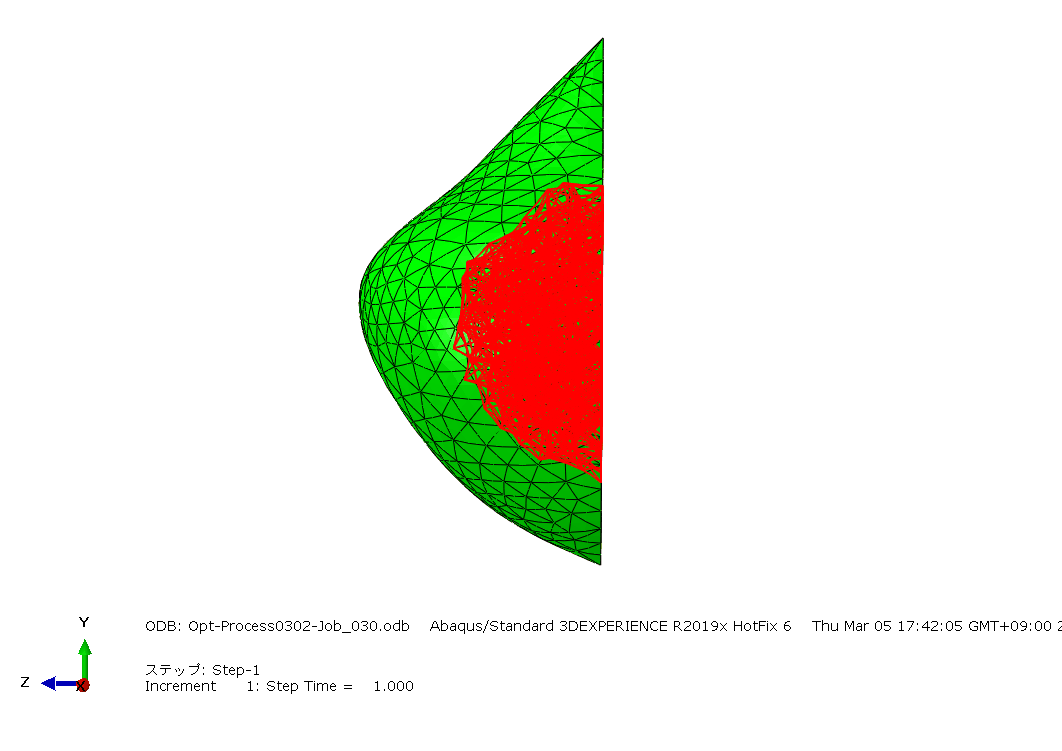
\includegraphics[width=0.8\columnwidth]{Figure/test.png}
			\caption{最適化結果(赤が最適化された乳腺)}
			\label{fig:ResultYZview}
		\end{figure}
		
		\begin{figure}[!h]
			\centering
			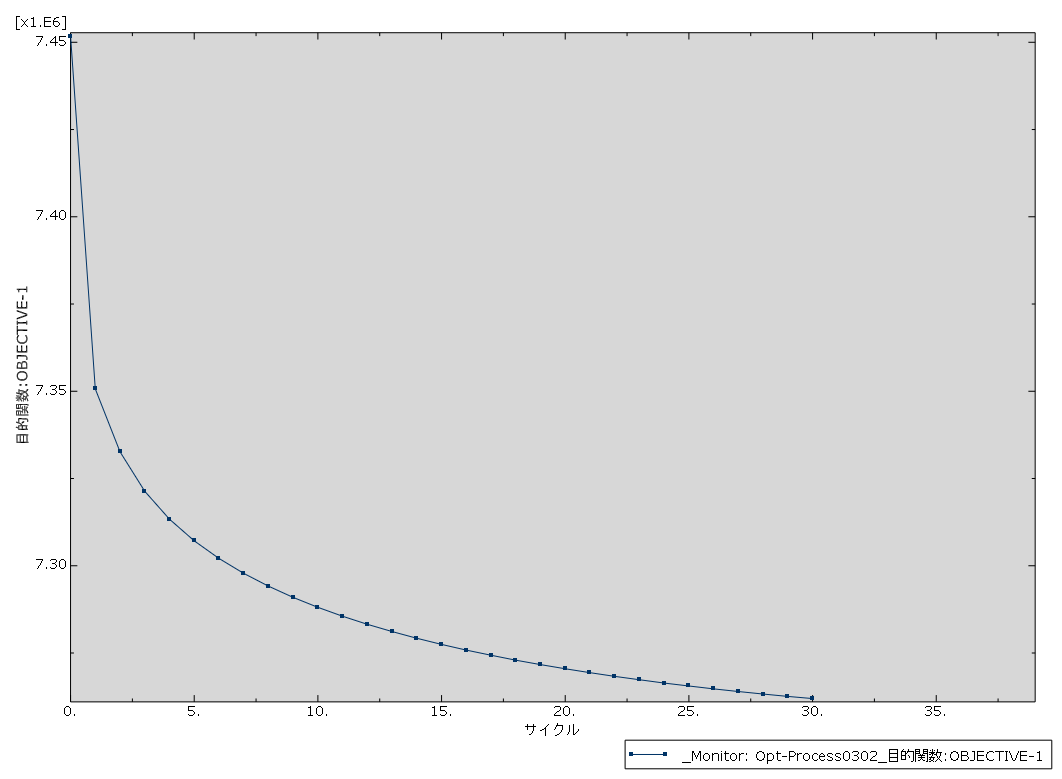
\includegraphics[width=0.6\columnwidth]{Figure/test2.png}
			\caption{イタレーションごとの目的関数の値}
			\label{fig:Graph}
		\end{figure}
	
	
	\newpage
\vspace{10cm}
%%%%%%%%%%%%%%%%%%%%%%%%%%%%%%%%%%%%%%
% 3.達成できなかったこととその問題点
	%\articleSPRthree
%%%%%%%%%%%%%%%%%%%%%%%%%%%%%%%%%%%%%%

\vspace{14cm}
%%%%%%%%%%%%%%%%%%%%%%%%%%%%%%%%%%%%%%
	\articleSPRfour
	\articleSPRfive
\end{document}
